\subsection{Elektronisch informiert}

Die wichtigsten Aufgaben der Studierenden sind der Besuch von
Lehrveranstaltungen, Zeitmanagement f"ur Studium und Freizeit und
Informationsbeschaffung. In diesem Artikel geht es um den letzten Punkt, und da
wir nun mal Informatik studieren, soll die Informationsbeschaffung "uber das
Internet erfolgen.

\begin{figure}[h]
  \centering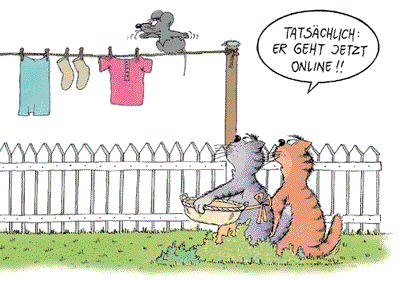
\includegraphics[width = \linewidth]{bilder/stein1.png}
\end{figure}

\subsubsection*{Adressen im World Wide Web}

Die Internet-Seiten der TU sind so riesig (oder un"ubersichtlich), dass man sie
auf den ersten Blick gar nicht begreifen kann. Ein paar Seiten der TU und
etliche Links aus dem restlichen WWW seien hier genannt.

 \begin{description}
 \item[TU-Homepage]~\\\nurl{http://tu-braunschweig.de/}
 \item[Hauptseite der Informatik]~\\\nurl{http://www.cs.tu-bs.de/}
 \item[Fachgruppenrat Informatik]~\\\nurl{http://fginfo.cs.tu-bs.de/}
 \item[Fachbereichssekretariat / Pr"ufungsamt]~\\
 \nurl{http://tu-braunschweig.de/fk1/service/informatik}
 \item[Mensa-Speisepl"ane]~\\
 \nurl{http://sw-bs.de/braunschweig/essen/}
 \item[BAf"oG-Amt]~\\\nurl{http://sw-bs.de/braunschweig/finanzen/}
 \item[Gauß-IT-Zentrum]~\\\nurl{http://tu-braunschweig.de/it}
 \item[Unisport]~\\\nurl{http://www.unisport.tu-bs.de/}
 \item[Sprachenzentrum]~\\\nurl{http://www.sz.tu-bs.de/}
 \item[Immatrikulationsamt]~\\\nurl{http://tu-braunschweig.de/i-amt/}
 \item[Stadt Braunschweig]~\\\nurl{http://braunschweig.de/}
 \item[Stadtplan f"ur Braunschweig]~\\\nurl{http://stadtplan.braunschweig.de/}
 \item[Campus-BS.de Portal]~\\\nurl{http://www.campus-bs.de/}
 \item[Stadtmagazine]~\\\nurl{http://www.subway-net.de/}
 \item[Schwimmb"ader in Braunschweig]~\\\nurl{http://www.stadtbad-bs.de/}
 \item[Kennelbad (Freibad \& Open-Air-Kino)]~\\\nurl{http://www.kennel-bad.de/}
 \item[Kinos]~\\\nurl{http://www.cinemaxx.de/}\\
   \nurl{http://www.bs-net.de/kino/}
 \item[MonkeyIsland]~\\\nurl{http://gruppen.tu-bs.de/monkeyisland/}
 \item[Schuntille]~\\\nurl{http://www.schuntille.de/}
 \item[Michaelishof]~\\\nurl{http://www.michaelishof.de/kneipe/}
 \item[Atelco, Karrenf"uhrerstr. 1-3]~\\\nurl{http://www.atelco.de/}
 \item[EGA.Com, Bohlweg 55]~\\\nurl{http://www.egacom.de/}
 \item[Kosatec, Kleine Burg 14]~\\\nurl{http://www.kosatec.de/}
 \item[SHV-Computer, B"ultenweg 81]~\\\nurl{http://www.shv-computer.de/}
 \item[Skycom, Gifhorner Stra"se 148]~\\\nurl{http://www.skycompc.de/}
 \item[Vobis, Otto-von-Guericke-Stra"se 2]~\\\nurl{http://www.vobis.de/}
 \item[Art of Systems, Wendenstrasse 58]~\\\nurl{http://www.artsys.de/}
 \end{description}

\subsubsection*{Mailinglisten}

Die wichtigste Mailingliste f"ur Informatikstudierende ist die Liste
\textbf{cs-studs}. Da bei den Wirtschaftsinformatikern oftmals auch
informatikrelevante Themen diskutiert werden, lohnt sich m"oglicherweise auch
ein Blick in \textbf{winfo-studs}. Wenn ihr an Stellenangeboten und Werbung aus
der freien Wirtschaft interessiert seid, steht die Mailingliste
\textbf{firmenkontakt} zu eurer Verf"ugung. Die Informatik-Kolloquien, das sind
Vortr"age von "ublicherweise externen Referenten zu Informatik-Themen, werden
auf der Mailingliste \textbf{kolloq} angek"undigt. Alle bisher genannten
Mailinglisten sind "uber \nurl{http://www.cs.tu-bs.de/mailinglisten.html}
erreichbar.

\subsubsection*{Newsgroups}

Die auf dem Newsserver \nurl{news://news.tu-bs.de} (nur aus dem TU-Netz heraus
erreichbar) liegenden Newsgroups werden leider nur sehr m"a"sig genutzt.
Mitteilungen des Rechenzentrums kommen "uber \textbf{tubs.general},
Mitteilungen speziell f"ur WLAN-Nutzer auf \textbf{tubs.wlan.d}. Die Newsgroups
\textbf{tubs.studium} und \textbf{tubs.studium-informatik} k"onnte man mal
wiederbeleben. Sehr reger Betrieb herrscht auf
\textbf{braunschweig.allgemeines} und der f"ur Schn"appchenj"ager idealen
\textbf{braunschweig.kaufrausch}.

\subsubsection*{IRC}

Im Freenode IRC (\nurl{http://freenode.net}) gibt es den Channel \nurl{##cs-studs}. Hier
sind immer ein paar BraunschweigerInnen und große Teile des Fachgruppe online. Die Gespr"achsthemen haben (im weitesten
Sinne ;) mit dem Studium zu tun.

